\documentclass{article}
\usepackage{scimisc-cv}
\usepackage{hyperref}
\usepackage{fancyhdr}
\usepackage{graphicx}
\usepackage{xcolor}
\usepackage[export]{adjustbox}
\title{ Mikhail Solovyanov CV for Electronic Positions}
\author{Mikhail Solovyanov}
\date{\today}
 
%% These are custom commands defined in scimisc-cv.sty
\cvname{Mikhail Solovyanov}
\cvpersonalinfo{
25 years old \cvinfosep
Yerevan, Armenia \cvinfosep
+374-44-190-197 \cvinfosep
solovyanov.mm@phystech.edu \cvinfosep
\href{https://www.linkedin.com/in/mikhail-solovyanov-b4a32b217/}{linkedin} \cvinfosep
\href{https://github.com/mikprin}{github}
}
 
%\rhead{\begin{picture}(0,0) \put(0,0){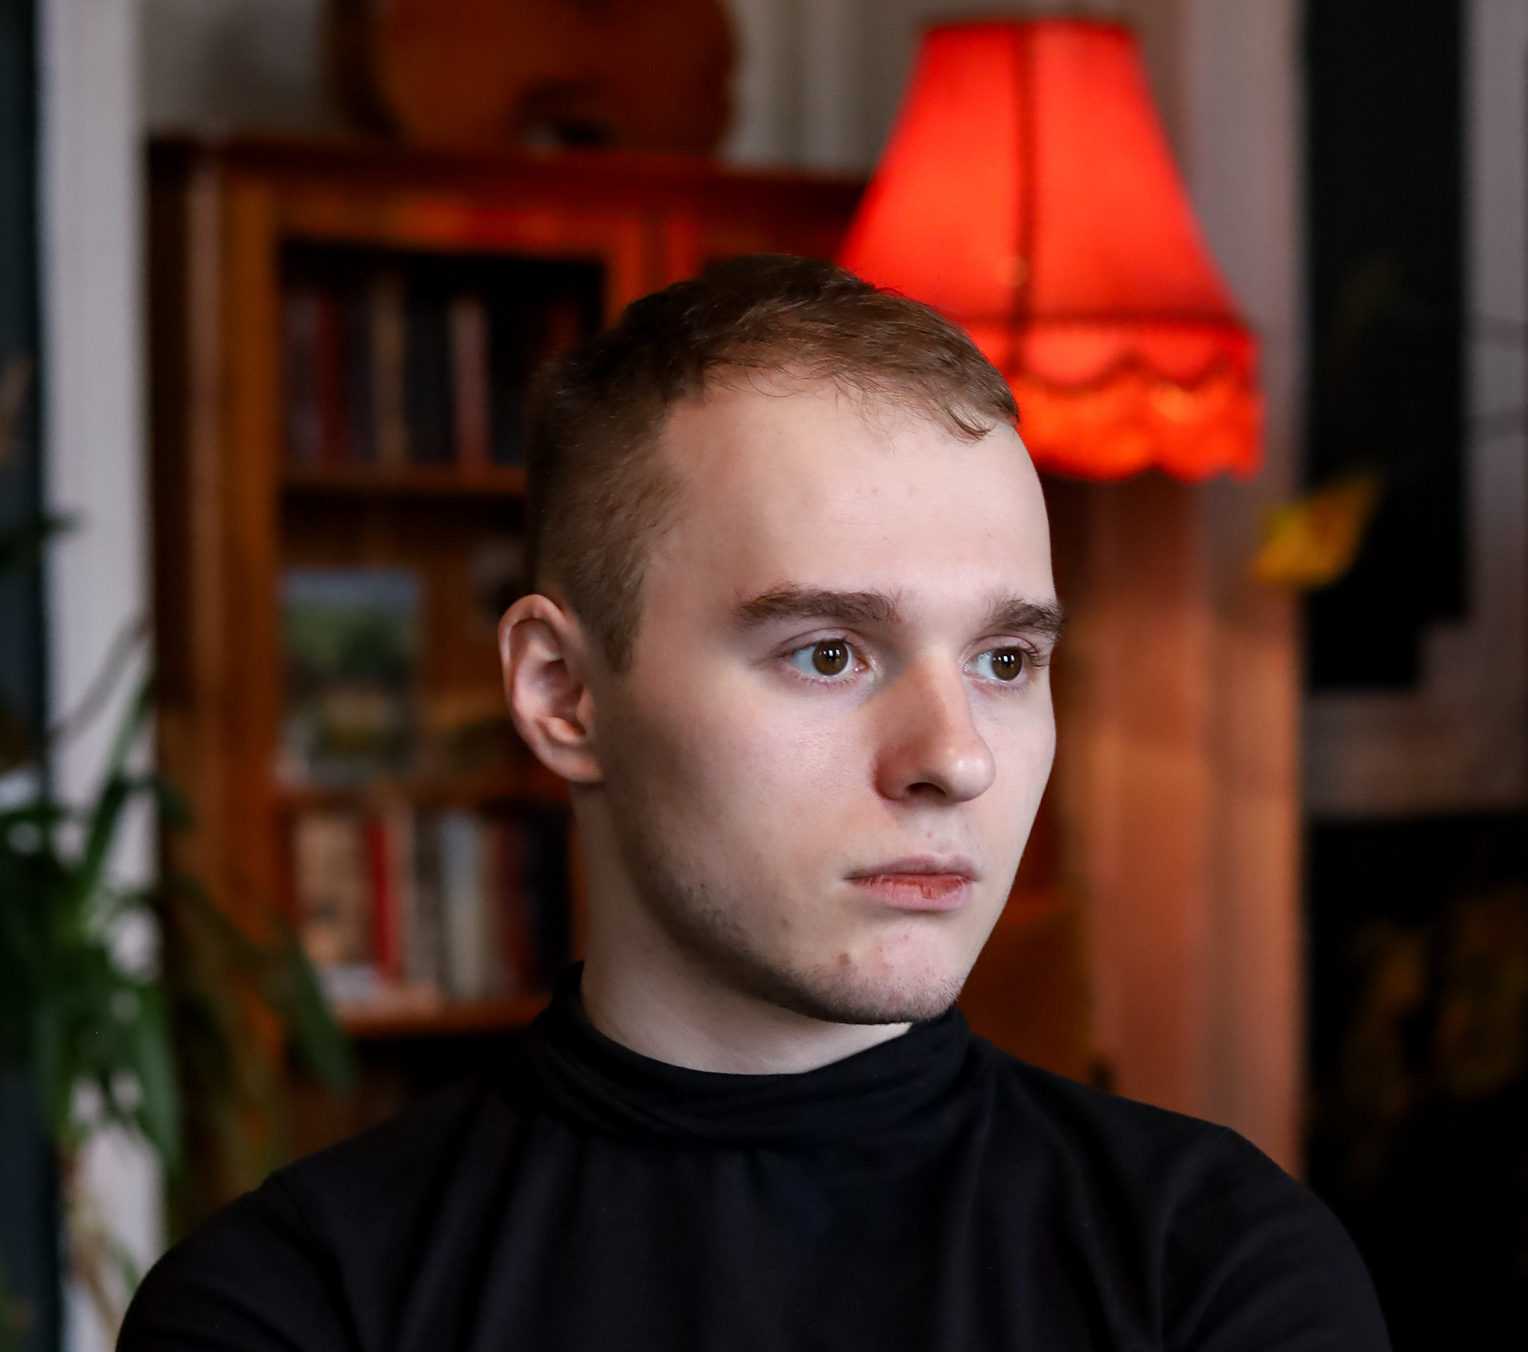
\includegraphics[width=1cm]{picture.jpg}} \end{picture}}

\begin{document}

% \maketitle %% This is LaTeX's default title constructed from \title,\author,\date
 
\makecvtitle %% This is a custom command constructing the CV title from \cvname, \cvpersonalinfo
%\smash{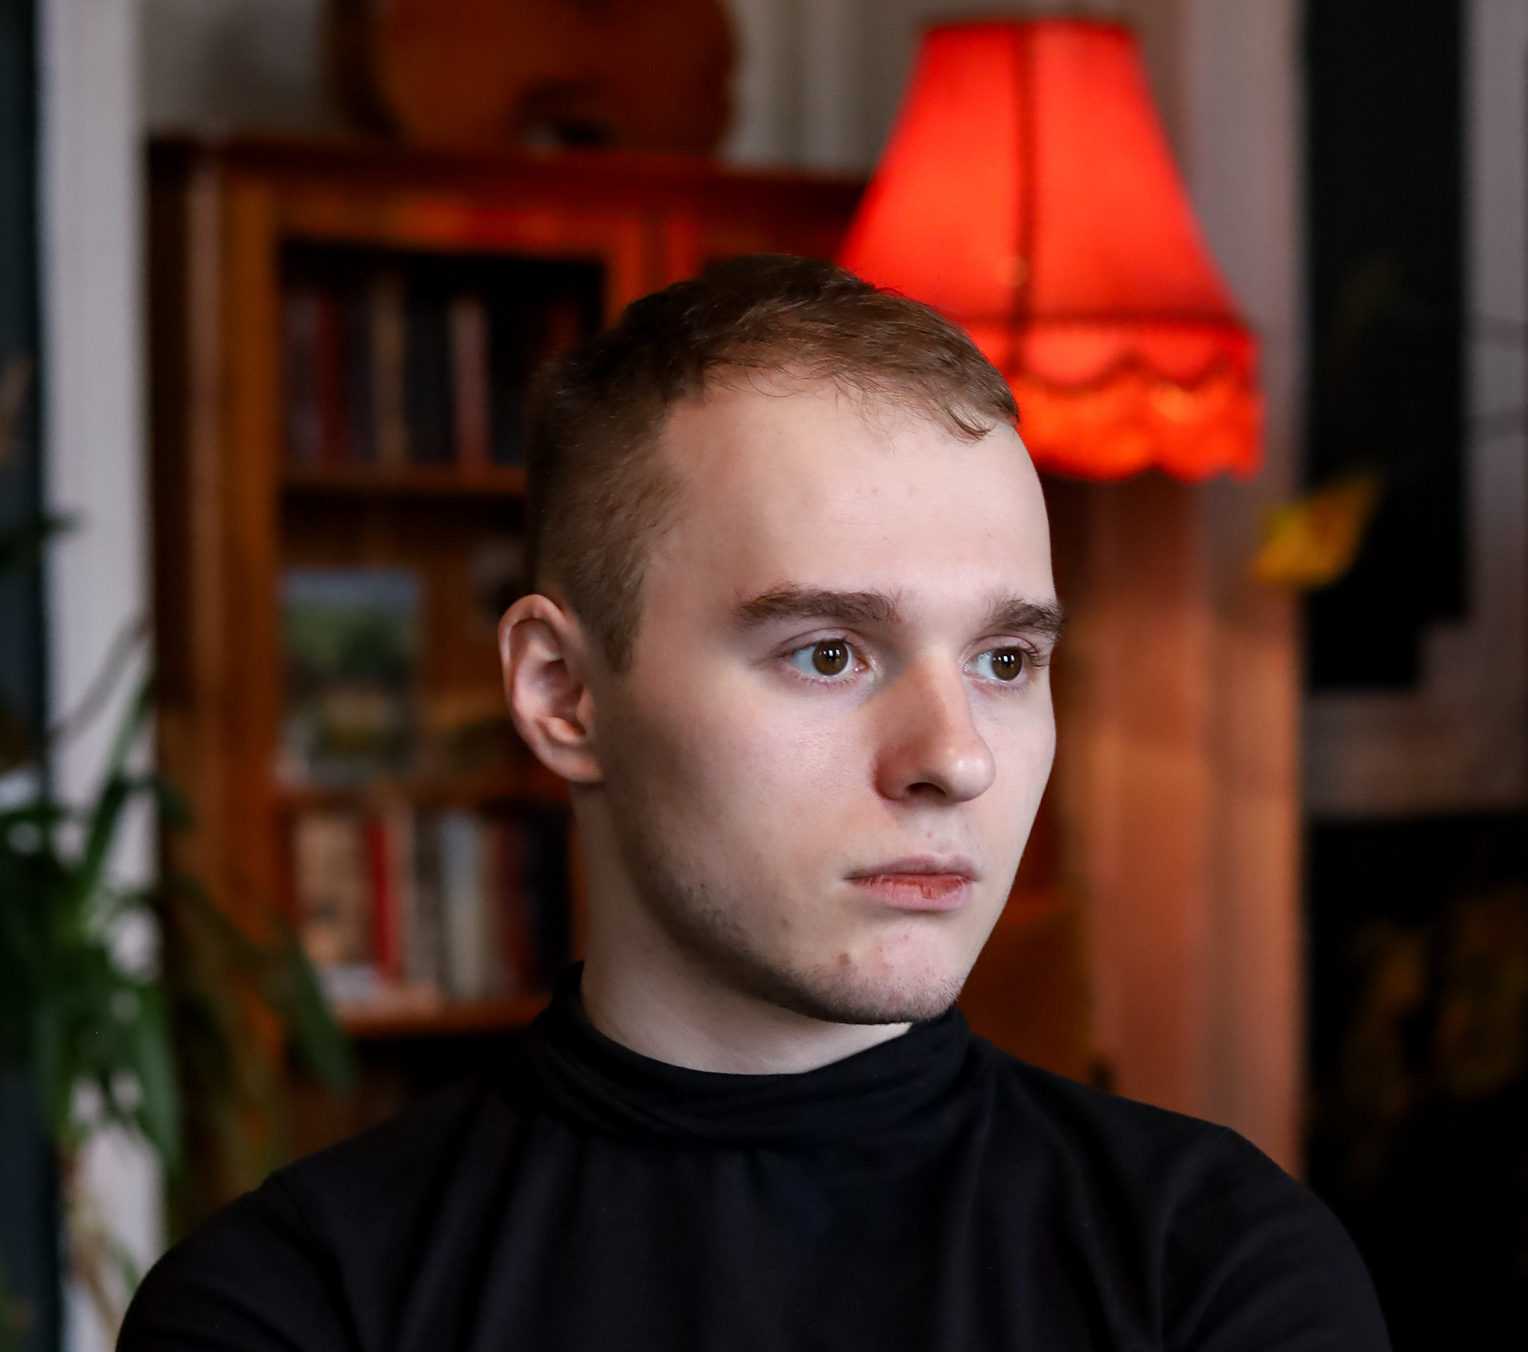
\includegraphics[width=3cm]{picture.jpg}}
%\raisebox{-.5\totalheight}[0pt][.5\totalheight]{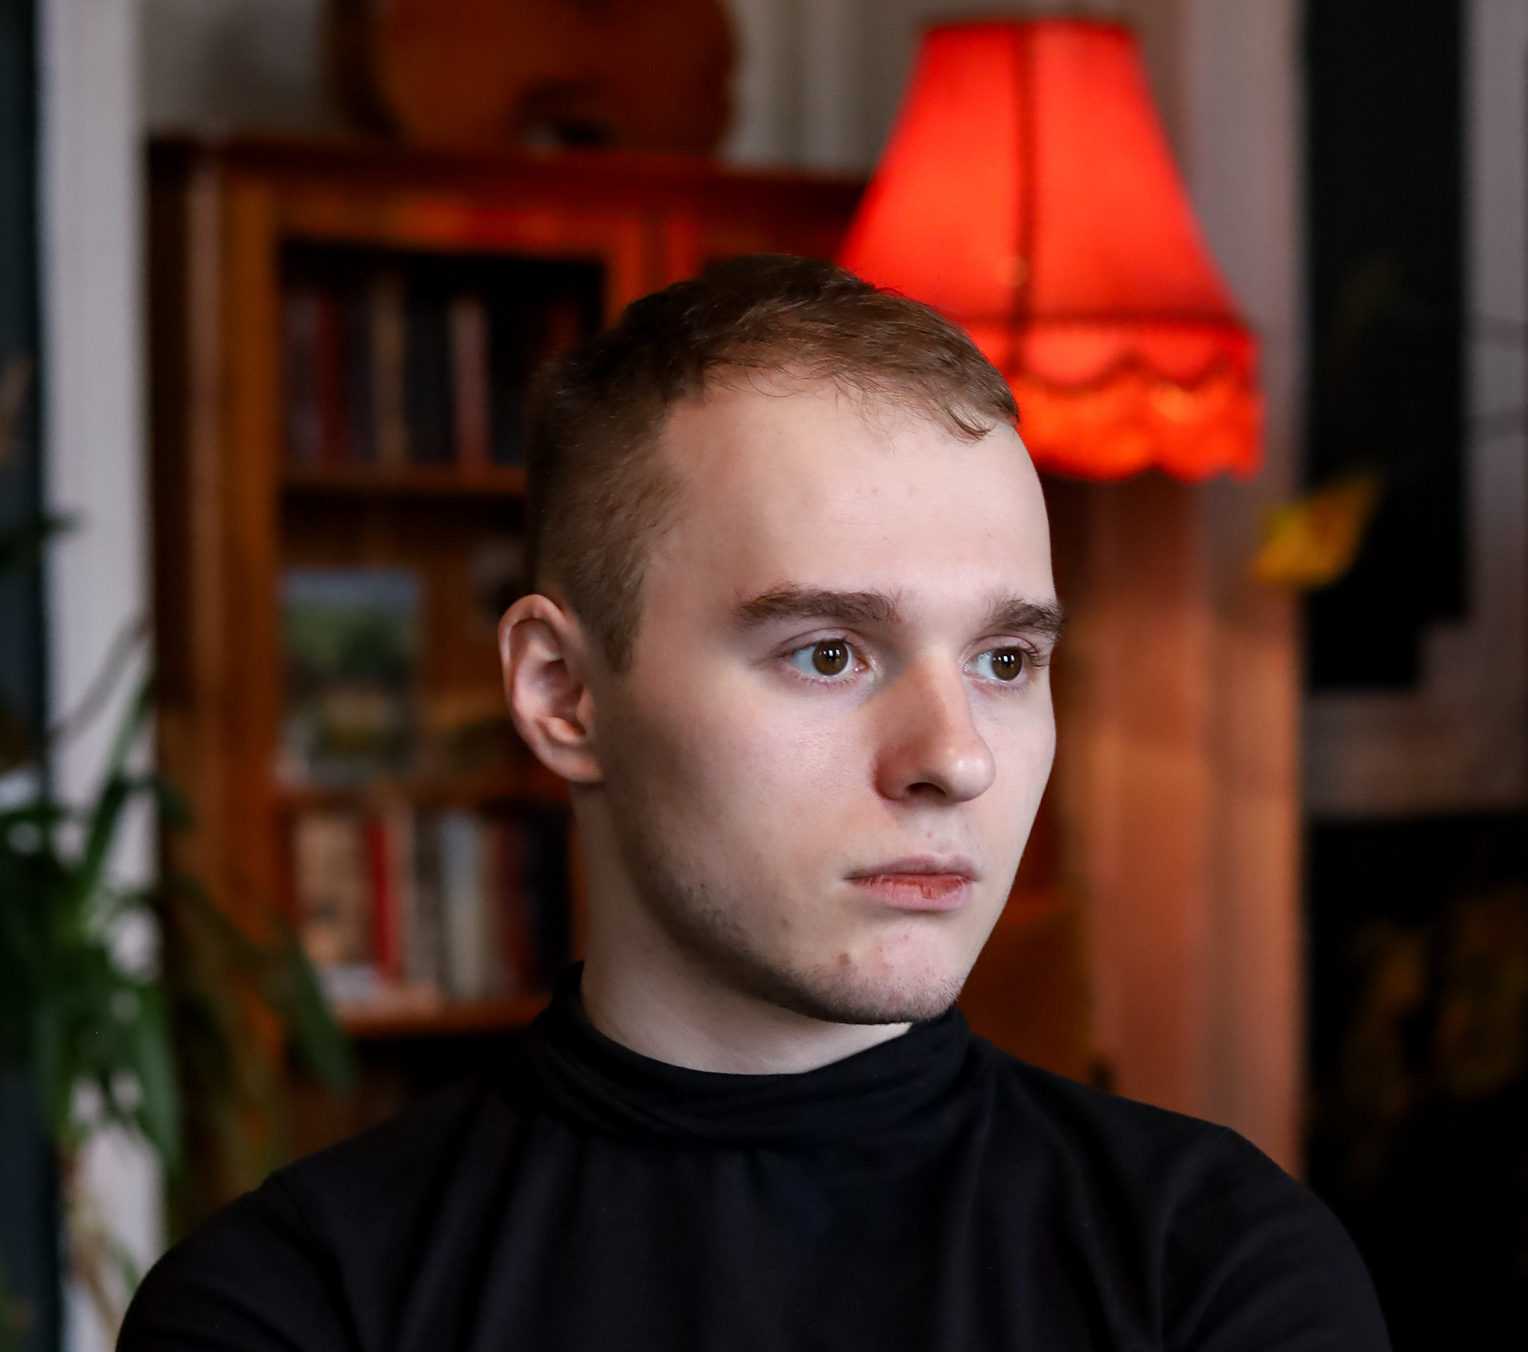
\includegraphics[width=10cm,height=10cm]{picture.jpg}}

\section{Summary}
\begin{minipage}{0.7\textwidth}
   \begin{itemize}
      \item Interdisciplinary electrical engineer, programmer and scientist with skills and experience in electronics, programming, machine learning, computer networks and measurements.
      \item Led development of a  project resulting in a patent.
      \item Self-motivated, problem-solving and collaborative scientist with notable communication and management skills.
      \item Have no stress digging in interdisciplinary fields and learning new subjects on the fly.
      \end{itemize}
   \end{minipage}%
   \hfill
   \begin{minipage}{0.3\textwidth}
      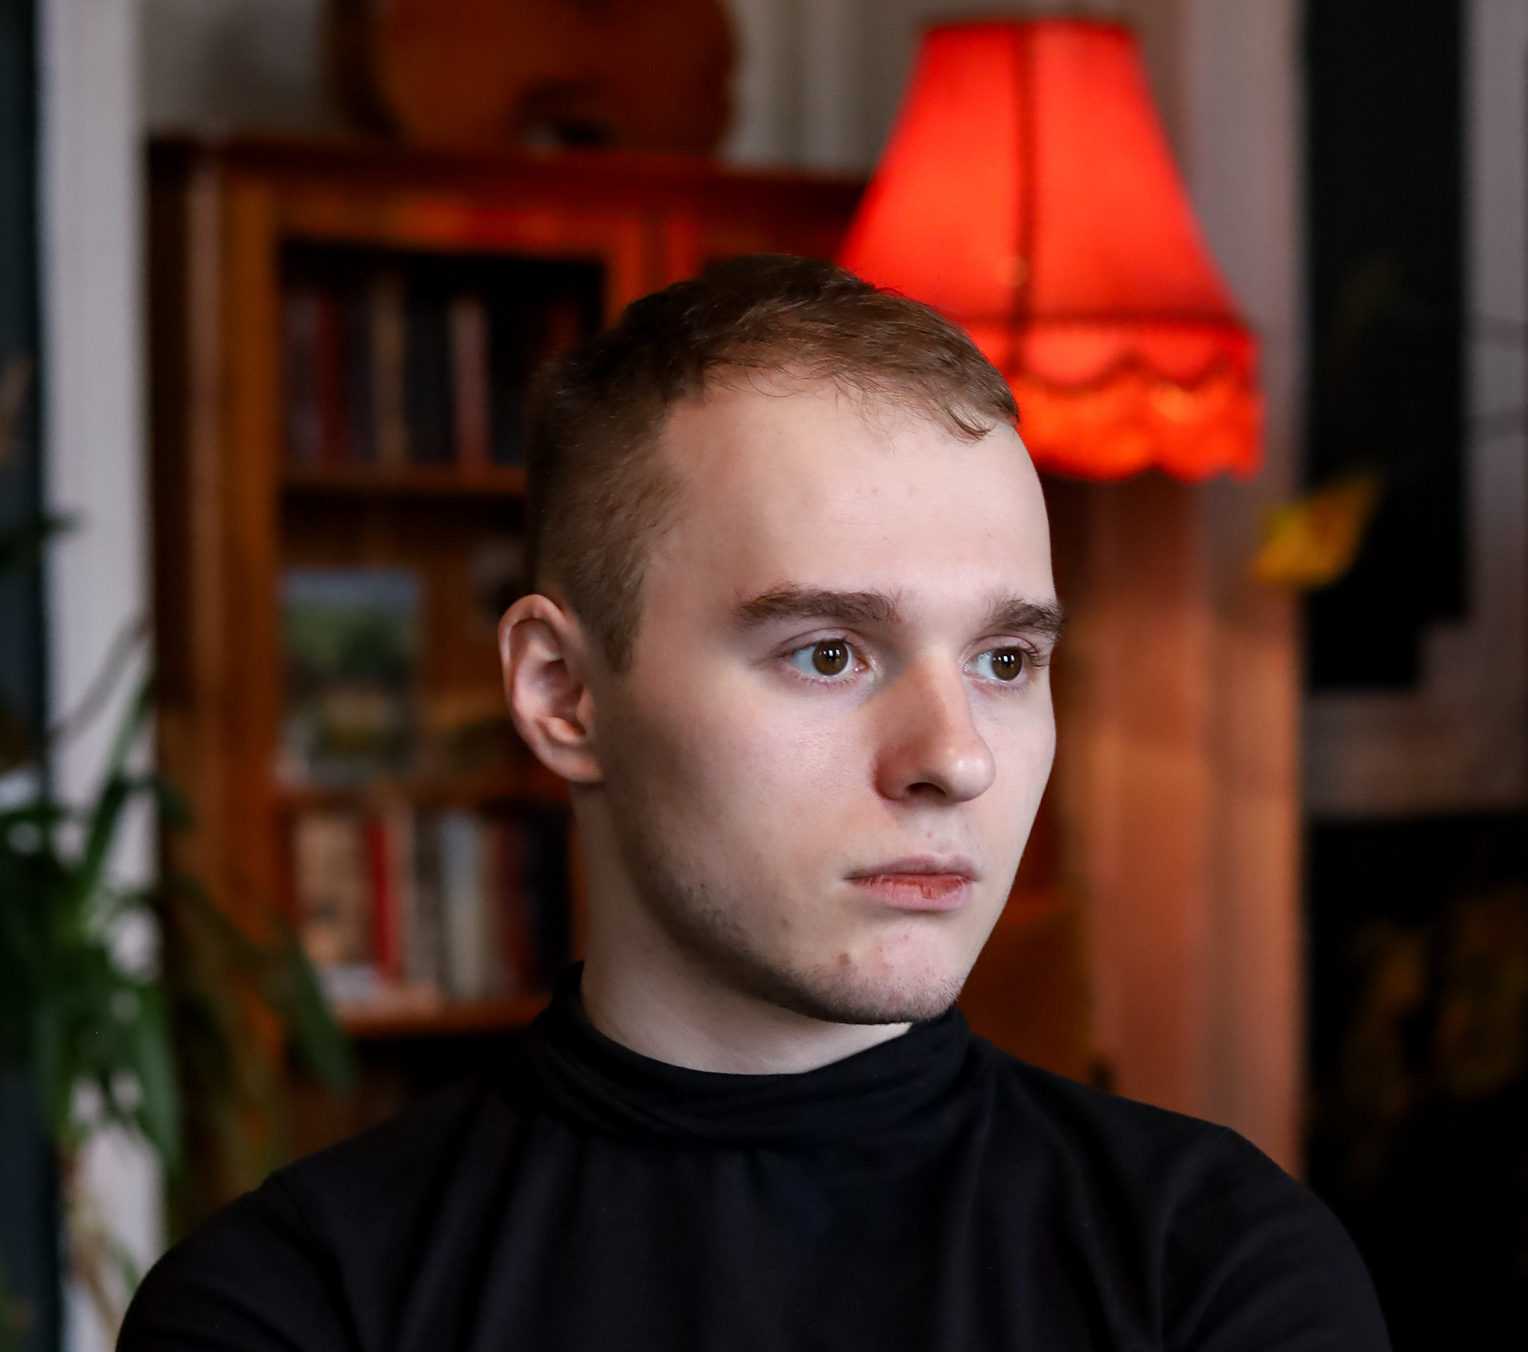
\includegraphics[width=3.5cm,right]{picture.jpg}
\end{minipage}%


% PICTURE ON THE LEFT
% \begin{minipage}{0.3\textwidth}
%    %\begin{tabular}{0.8\textwidth}{\raggedleft\arraybackslash}
%       %\begin{figure}
%          %\begin{figure}
%             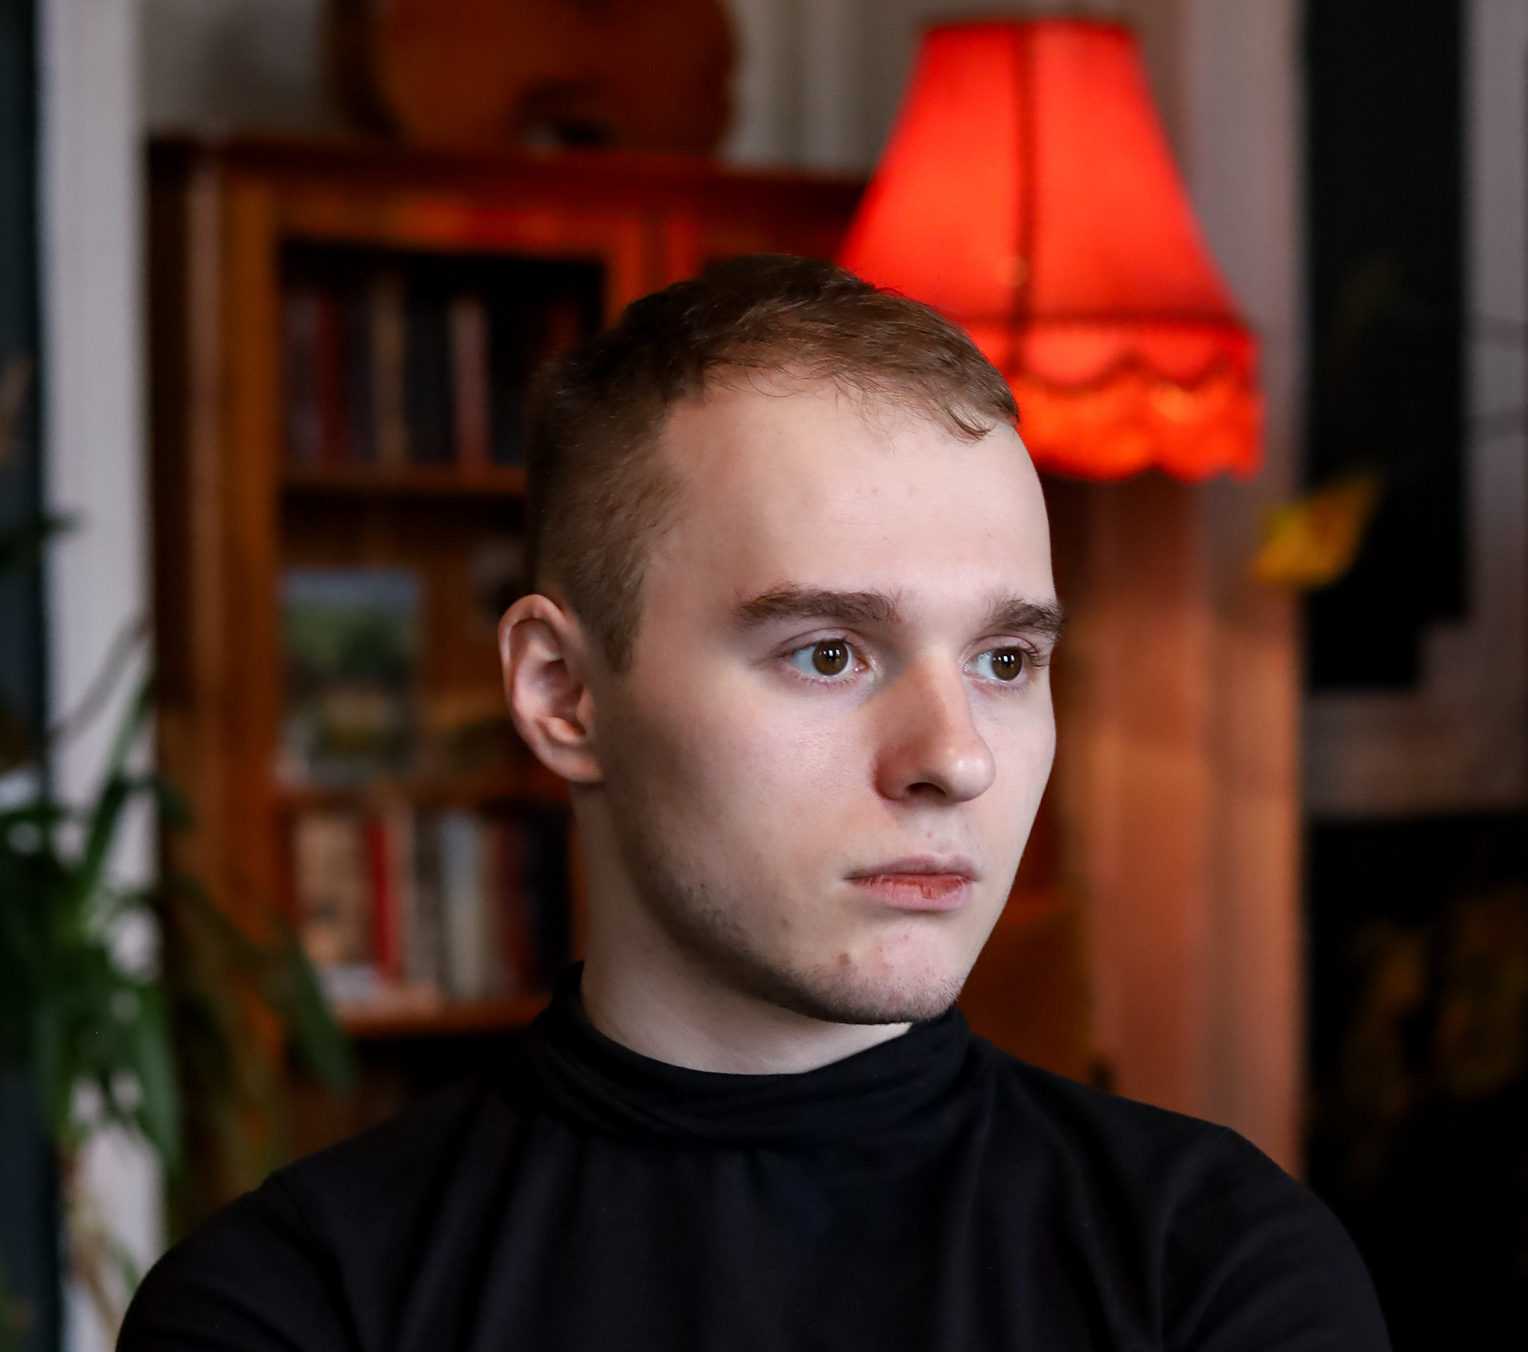
\includegraphics[width=4cm,left]{picture.jpg}
%         %\end{figure}
%       %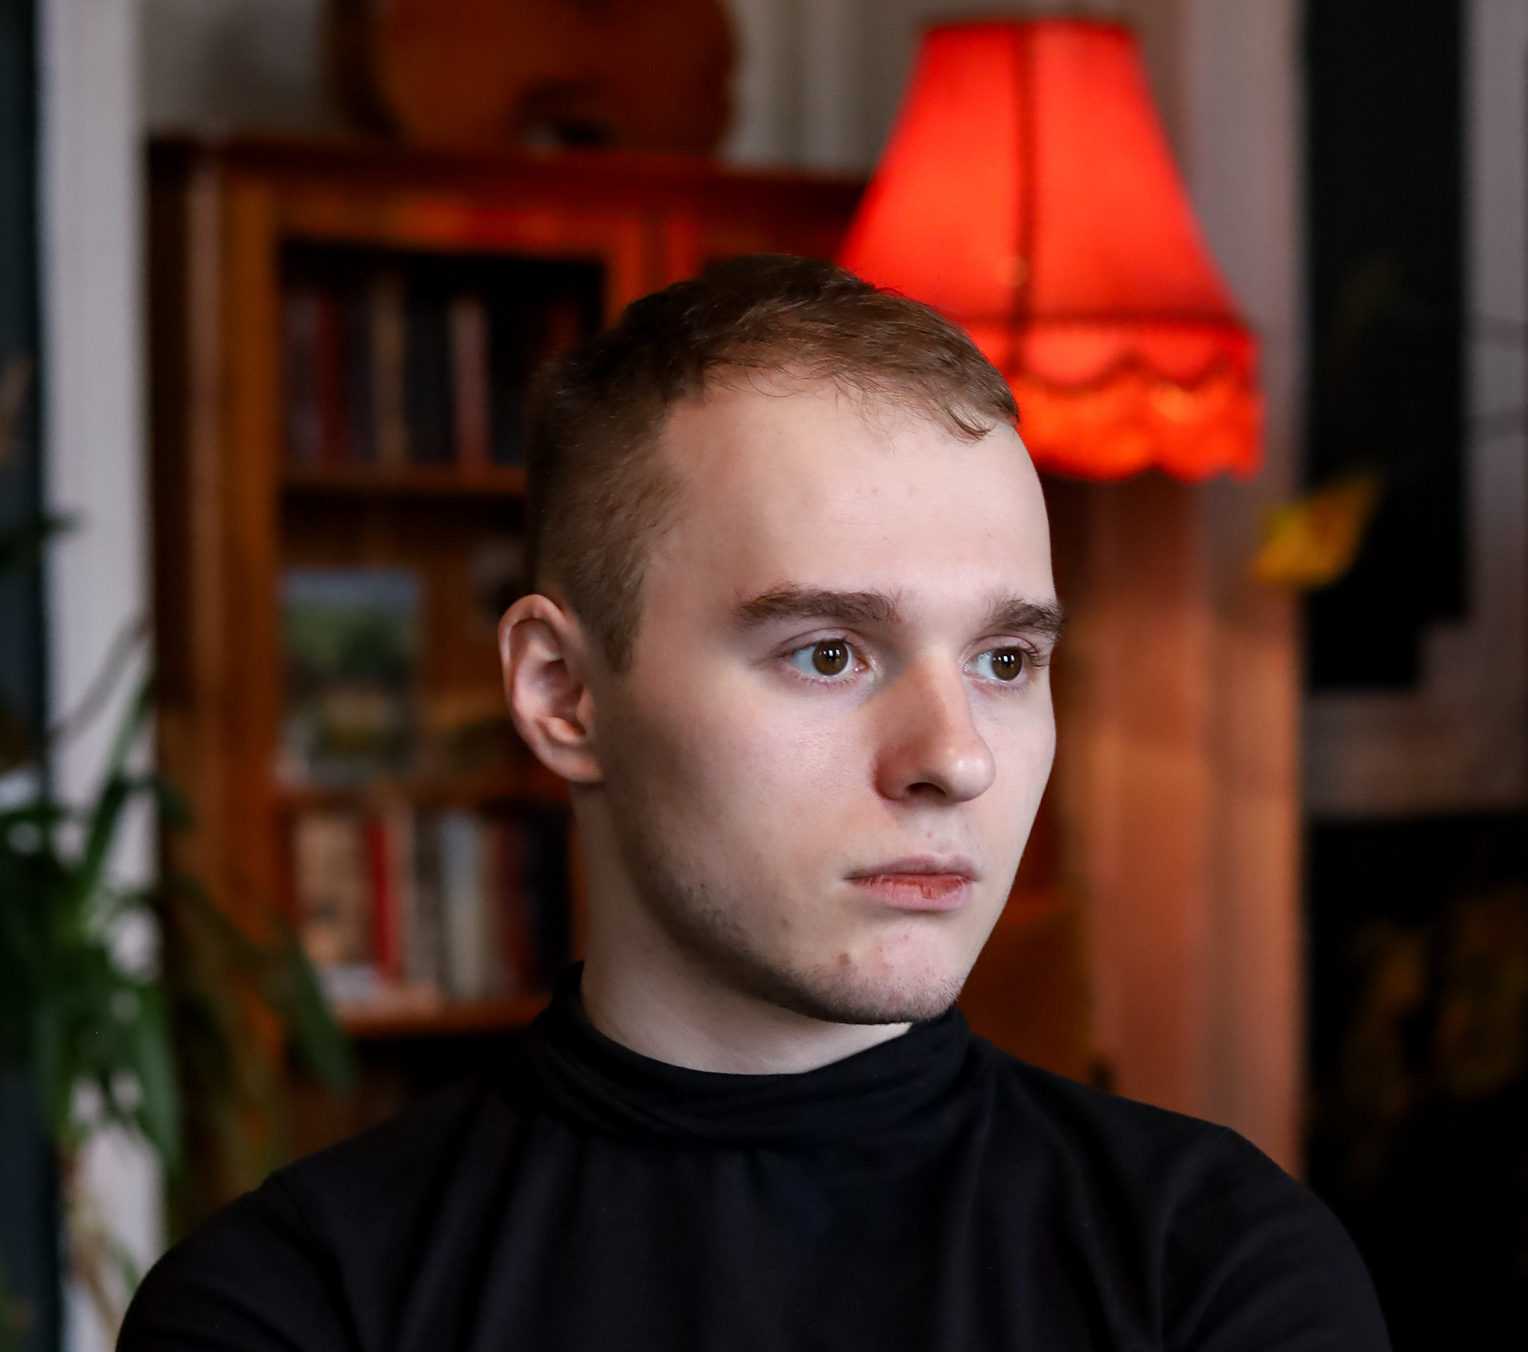
\includegraphics[width=4cm,right]{picture.jpg}  
%       %\end{figure}
%    %\end{tabular}
% \end{minipage}%
% \hfill
% \begin{minipage}{0.7\textwidth}
%    \begin{itemize}
%       \item Interdisciplinary electrical engineer, programmer and scientist with skills and experience in electronics, programming, machine learning, computer networks and measurements.
%       \item Led development of a  project resulting in a patent.
%       \item Self-motivated, problem-solving and collaborative scientist with notable communication and management skills.
%       \item Have no stress digging in interdisciplinary fields and learning new subjects on the fly.
%    \end{itemize}
% \end{minipage}%

% BEGIN OF RESUME

\section{Technical Skills}
 
\begin{itemize}

\item \textbf{Electronics IC design:} Analog and mixed IC Design. Signals and systems, control design, Memory design and simulation, digital Electronics simulation, experience simulating and working with ferroelectric capacitors and memristors (cells of ReRAM memory),   mixed signal simulation, \textit{AC,DC,PZ,transient} simulation, parasitic parameters analysis. Simulation and verification automation. Operational amplifiers, comparators, DAC, ADC design. Experience of making layouts for $65 nm$, $90nm$, $180nm$ nodes. Basic FPGA programming.
\item \textbf{Electronics PCB level design:} Full stack PCB design from schematic or device idea to SMT Assembly including Design for manufacturing (DFM). Embedded systems design (STM32,ESP32), raspberry pi, DSP, SDR,  control systems engineering , DC-DC converters, drivers, analog electronics, RF, IOT stack, impedance matched design, audio design.
\item \textbf{Software engineering:} General experience of collaborative functional and object-oriented programming. Working with data and data analysis. Data visualization. Basics of web development.
\item \textbf{Computational and Machine Learning, computer vision:} Applied machine learning algorithms. General knowledge in ML framework programming. General knowledge of machine learning methods. Optimization algorithms and basic CV algorithms.
\item \textbf{Networks and Computer engineering and administration:} Deep Linux knowledge, and be very comfortable working in various Linux environments as well as with Windows. Server and PC building for complicated tasks, building custom racks and networks, Firewall and network setup, containers management and automation, deployment of VPN and other server client oriented soft.
\item \textbf{Microscopy/Imaging/Materials:} Measuring equipment (oscilloscopes,VNA). SEM (Scanning Electron Microscope), Optical Microscope, lithography, ellipsometry, IC development lab processes, semi-professional Photography.
\item \textbf{Mechanical skills:} Soldering (including 0403 SMD), connector crimping,  assembling and general mechanical engineering knowledge and experience. 3D slicing and Printing.
\end{itemize}
 
\section{Software and Hardware Skills}
\begin{itemize}
\item \textbf{Programming langauges:} Python, C/C++, bash, VerilogA, MATLAB, Simulink, SimScape, Verilog, gnuradio. 
\item \textbf{Electronics IC design:} Cadence virtuoso, SPICE, SPECTRE, Vivado, Vitis IDE.
\item \textbf{Electronics PCB and embedded design:} Altium designer, KiCad, LtSpice, also for Embedded tools: STM32 cube IDE, Arduino IDE, PlatformIO, ESP-IDF.
\item \textbf{DevOps and OS:} Docker, Ansible, Kubernetes, Linux, GIT.
\end{itemize}

\section{Research and work Experience}
 
%% Another custom command provide by scimisc-cv.sty.
%% First two arguments are typeset on the first line in bold; 3rd and 4th arguments are typset on second line in italics. 2nd, 3rd and 4th arguments are OPTIONAL

 
\cvsubsection{ \href{https://en.wikipedia.org/wiki/Synopsys}{Synopsys}}[Inc]
[Senior R\&D engineer][March 2022 to present]
   \begin{itemize}
      \item Development of FPGA based SMS and SHS memory testing solutions on Xilinx Zynq boards.
      \item Implementation of FPGA based prototype solution on Zynq device, including development of Firmware, RTOS, and Linux software to contact custom RTL code for memory testing. 
   \end{itemize}

\cvsubsection{ \href{http://twin3d.pro}{Twin3d}}[LLC][Leading electrical/software engineer][January 2021 to Feb 2022]
\begin{itemize}
   \item Built electrical and software system to trigger and access 240 DSLR cameras in time window of 10us. This biggest rig in Russia was made for making top edge 3D photorealistic models of people and animals for VFX, games, cinema etc.
   \item Developed custom IOT solution build around raspberry pi and ESP32 to control 240 cameras, lights and 10 controlling computers and controllers with USB, UART, TCP, MQTT and SSH protocols.
   \item Eventually managed team of 2 programmers and 2 mechanical engineers for making scanners upgrades.
   \item Built and maintained company IT infrastructure including servers for four RTX 3090 graphics cards for ML load and more.
   \end{itemize}

\cvsubsection{\href{https://mipt.ru/english/}{MIPT Neurocomputing systems lab}}[BS + MsC]
[Engineer][September 2017 to September 2021]

\begin{itemize}
\item This project coordinated by  \href{https://www.scopus.com/authid/detail.uri?authorId=56272708000}{D.Negrov}   led to development of IC's with a $Hf_{0.5} Z_{0.5} O $ based  FRAM with 5nm thin ferroelectric layer.
%\item This project led to 2 conference theses.
\item Responsible for development of a prototype of a memory  compiler for new FRAM or ReRAM memory (Python and bash).
\item Last year of work led to completion of essential analog components for memory testing chip. Developed comparators and Op Amps for ADC and DAC as part of SMU system on a chip.
\item Used machine learning methods to evaluate parasitics in prototype IC chips and measuring probes.

\end{itemize}
 

 
\cvsubsection{ \href{http://uvl.io/ }{UVL Robotics}  }[LLC]
[Electronic engineer / DevOps][Feb 2020 to Dec 2020]
 
\begin{itemize}
\item Responsible for development and programming of a motherboard PCB for AI based drones.
\item Created scripts for automated soft building on ARM64 Jetson Xavier NX computer.
\end{itemize}
 
 
%% An example of leaving an argument empty
\cvsubsection{Tech Agent Startup}[][Electronics Engineer][September 2019 to July 2020]
 
\begin{itemize}
\item Developed method to generate electrical impulses read by contact pulse-meter as human pulse. 
\item Developed commercial electronic device to work with almost any training apparatus. PCB design and Embedded C development for the device with BLE functionality. 
\item These projects led to the submission of a patent.
\end{itemize}
 
%% An example of leaving an argument empty
\cvsubsection{\href{https://ailiton.ru/en/}{Ailiton} medical research}[Unimed Group LLC][Electronics Engineer (as invited specialist)][July 2018 to December 2018]
 
\begin{itemize}
\item Led project focused on the developing a device to read a gel card using machine learning algorithms. Eventually, led to the creation of a commercial electronic device.
\end{itemize}
 
 
\section{Education}
 
\begin{itemize}
\item Masters, applied physics and math, Moscow Institute of Physics and Technology (MIPT) department of quantum and physical electronics, 2019-2021
\item BS, Bachelor of applied physics and math, Moscow Institute of Physics and Technology (MIPT) department of quantum and physical electronics, 2015-2019.
\end{itemize}

\section{Teaching and Mentoring Experience }
\begin{itemize}
\item 2021 Led Laboratory work (creation of Schottky diode) on the department of solid-state physics of MIPT. 
\item 2015-2019 - Mentored 6 undergraduates in their day-to-day physics and math SAT-level exam prep.
\item 2017-2018 - Tutoring in summer camps (foxford.ru)
\end{itemize}
 
\section{Awards and other}
\begin{itemize}
\item Have a \href{https://www.youtube.com/channel/UCAjmXQnYQjWoVHx6NIo24CQ}{YouTube Channel} about electronics and software.   
\item Winner of The 62th MIPT Scientific Conference, in section of nanotechnologies.
\end{itemize}
 
\section{Conference Presentations }
 
\begin{itemize}
\item \href{https://microelectronica.pro/}{International forum microelectronics 2019}. Thesis: "Developing high energy efficient FRAM memory in neurocomputing application".
\item  \href{https://conf62.mipt.ru/}{The 62th MIPT Scientific Conference.}. Thesis "Compiler for high energy efficient FRAM memory in neurocomputing application"
\item \href{https://mipt.ru/science/5top100/education/courseproposal/%D0%A4%D0%AD%D0%A4%D0%9C.pdf}{The 63th MIPT Scientific Conference.}. Thesis: "Development of SMU IC for testing energy efficient memories"
\end{itemize}
 
%\section{Publications}
%Still yet to come %
 
\section{Other Skills}
\begin{description}[widest=Langauges]
\item[Software]  Photoshop, InkScape.
\item[Languages] English: professional proficiency.  Russian: native.
\item[Photography] Have experience in professional photography.
\item[Hobbies] Making audio effects. Competition level dancer (WCS, Hustle), Making Educational content.
\end{description}
 
\end{document}